\subsection{Transformation}
\label{subsec:compilation}
%XSeparation generates object-oriented code containing additional constructs for bidirectional traceability. Hence, a compilation process is needed to transform the XSeparation-generated code into machine code.
The transformation transforms the intermediate code into the \tb{Standard code}. %to transform the XSeparation-generated code into machine code.
Fig. \ref{fig:compilerarchitecture} shows the transformation process.
The latter consists of two grayed sub-transformations: \tb{Structure code transformation} (SCT) and \tb{Behavior code transformation} (BCT). 

\begin{figure}
	\centering
	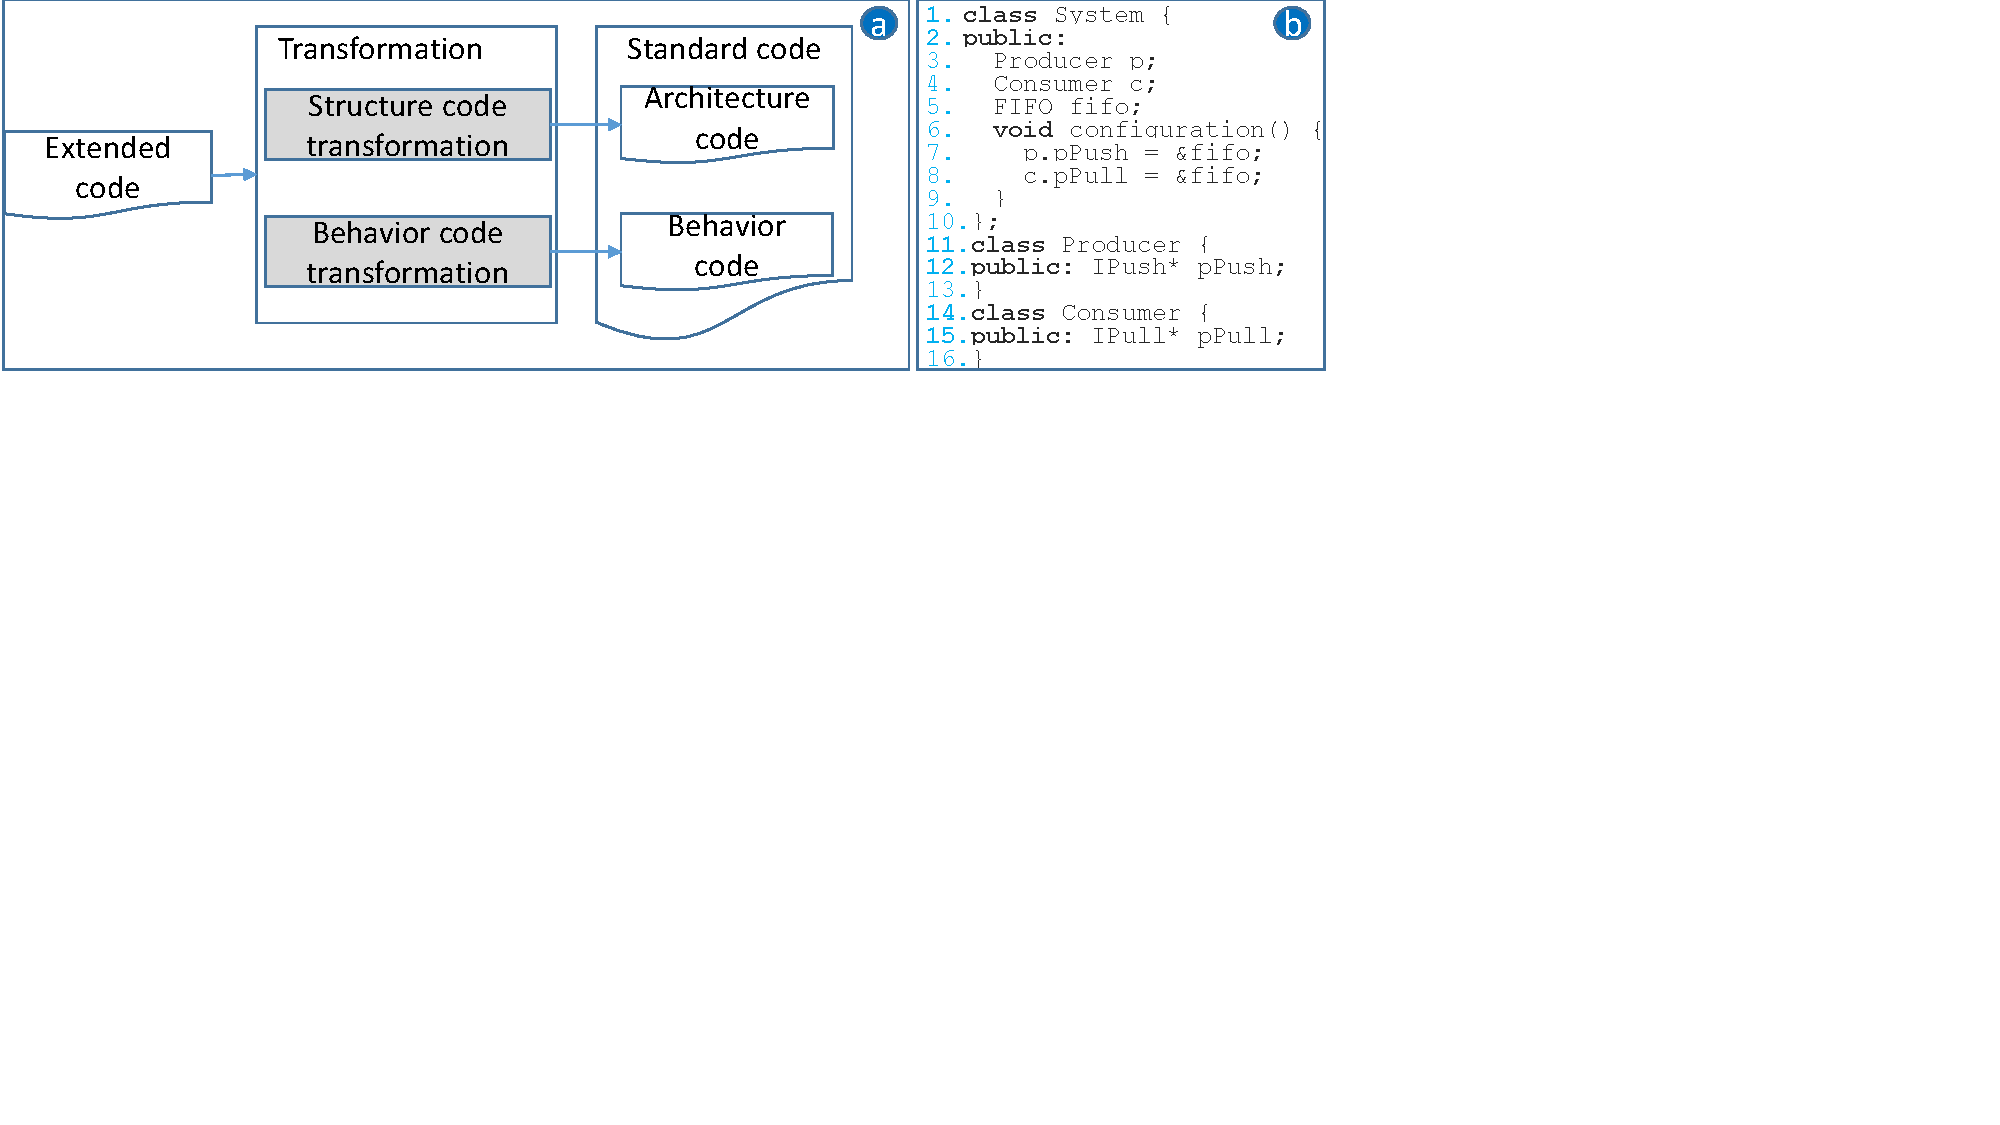
\includegraphics[clip, trim=0cm 12.6cm 10.7cm 0cm, width=\columnwidth]{figures/compilerarchitecture-code.pdf}
	\caption{XSeparation compiler's architecture} 
	\label{fig:compilerarchitecture}
\end{figure}

%\vskip 0.1cm
\noindent
\tb{Structure code transformation:}
%A verification is firstly executed to check the well-formedness of components and ports.
%We basically verify three port rules: (1) every port with a required interface or provided data must be bound to another port; (2) if two ports are connected by a assemble connector, the provided interface/data of one port must identical to or an extension of the required interface/data of the other port; and (3) if the connector is delegate, the provided interface/data of one port must identical to or an extension of the provided interface/port of the other port; 
%Once the rules are verified, executable code can be generated. 
SCT transforms the additional structural constructs into standard code.
Fig. \ref{fig:compilerarchitecture} shows a segment of standard code generated from the producer-consumer example.
Each port with required interface is transformed into a pointer attribute (lines 12 and 15) while each part into an object attribute (lines 3-5).
%A configuration method is transformed into a method \ttt{configuration}.
A binding (bindPorts) in the configuration is transformed into an assignment which refers the pointer associated with a port with provided interface to the corresponding implementation.
For example, the \ti{pPush} pointer of \ti{Producer} is referred to the fifo, which implements the \ti{IPush} interface (line 7). 
When a method is called through a port, for example \ttt{push} through the \ttt{pPush} port, the corresponding method implemented in FIFO is invoked. 


%\vskip 0.1cm
\noindent
\tb{Behavior code transformation:}
It transforms the behavioral constructs for state machines into standard code similarly to code generation approaches from UML State Machines in MDE tools such as Rhapsody.
Our goal is to support all of the features of state machines.
However, the existing tools only support a subset of state machine concepts, e.g. Rhapsody does not support junctions, truly concurrent execution of orthogonal regions \cite{ibmdiff}, and all of the UML event types.
%UML events are not supported 
%The concurrency of the orthogonal regions is often implemented sequentially \cite{Badreddin2014}. 
%In addition, there are other issues such as event processing speed, executable file size, and UML semantic-conformance defined by a recent work on the Precise Semantics of State Machine (PSSM) \cite{OMG2015}.
%XSeparation compiler supports full features of state machines.
%XSeparation compiler has following features.

%\begin{itemize}[\footnotesize]
We extend an existing code generation pattern with the use of IF/ELSE to support all of the state machine features. 	
%We currently evaluate the semantic-conformance of  A recent specification formalizing the precise semantics of UML State Machine is under standardization of OMG.
%It defines a test suite with 66 test cases for certifying the conformance of runtime execution of code generated from UML State Machines.
%We have experimented XSeparation compiler with the test suite.
%The traced execution results of 62/66 test cases comply with the standard and are a good hint that the execution is semantically correct.
Due to space limitation, the details of pattern and evaluation for state machine runtime execution semantics are not presented in this paper.

%\vskip 0.1cm
%\noindent	
%\tb{State machine configuration:} XSeparation allows to configure the event queue size and periodic time for evaluation of change events.

%\vskip 0.1cm
%\noindent	
%\tb{Event API:} Generated code in XSeparation compiler provides APIs for environment code to invoke operations or send data signals through component ports.
%	The invocations and sending will automatically fire events for state machines to process.
%\end{itemize}

%\vskip 0.1cm
%\tb{Runtime}
%Asynchronous events are stored in an event queue managed by the component at runtime.
%Furthermore, the boolean expression of ChangeEvent is periodically evaluated.
%The size of the queue and the periodic evaluation time can be configured within the topology of the state machines.
%Others such as event priorities are configurable but not implemented for the moment.
%Lines 32-35 in Listing \ref{lst:fifostatemachine} configures the size of the queue as 50 and the periodic evaluation time is 20 millisecond.
%Note that this configuration is different from the structure configuration, which is used for wiring different components through explicitly defined ports.
%UML, however, remains abstractly and does not specify these configuration values.
%We then define a profile support for UML State machine configuration.
%Fig. \ref{fig:fifostatemachine} shows the configuration values annotating the state machine example.

%In the next section, XSeparation will be implemented as an extension of the Papyrus modeling tool and evaluated by developing a case study of software application for LEGO.